\documentclass[conference, compsoc]{IEEEtran}

\usepackage{graphicx}
\usepackage[UKenglish]{isodate} % for dmy date
\usepackage{blindtext}
\usepackage{fancyvrb} % for code

\RequirePackage[singlelinecheck=off]{caption}
\captionsetup{justification=centering}

\title{\huge{LoRa PHY Range Tests and Software Decoding}}
\cleanlookdateon
\author{Keely Hill\\\today}

% fixes bib use
\def\endthebibliography{%
  \def\@noitemerr{\@latex@warning{Empty `thebibliography' environment}}%
  \endlist}

\begin{document}

\maketitle

\begin{abstract}
LoRa is a recently created patented physical layer protocol for small, low power devices. Networks are being deployed world wide as LoRa WAN (link layer). The attack surface is growing. This project begins by performing range tests of a consumer module physical (PHY) layer. Depending on the settings, up to 5 Km was achieved to transmit a frame -- at the expense of speed. 1 Km was achieved at a more reasonable rate. Along the way, how LoRa functions is discussed. Next and inexpensive RTL-SDR (software defined radio) was used to record raw transmissions from the official PHY module. These transmissions were then attempted (and successfully) demodulated and decoded using GNU Radio and the experimental gr-lora out-of-tree module from Bastille Reasearch. Some common radio vulnerabilities are discussed in relationship with LoRa as a conclusion.
\end{abstract}

\renewcommand\IEEEkeywordsname{Keywords}
\begin{IEEEkeywords}
LoRa, range testing, Software Defined Radio (SDR), physical layer security
\end{IEEEkeywords}

%%%%%%%%%%%%%%%%%%%%%%%%%%%%%%%%%%%%%%%%%%%%%%%%%%%

\section{Introduction}
This is an experimentation project performed with the LoRa physical layer (PHY) using an official consumer LoRa device and software defined radio (SDR). Range testing and successful SDR decoding attempts are performed. As LoRa device networks are deployed around the world, the attack surface grows. It is important to understand what these low powered devices are capable of, and how they function.

\section{LoRa Overview}
LoRa is a patented physical layer chirp spread spectrum modulation format. LoRa operates in license-free bands (433 MHz in Europe, 915 MHz in the US). LoRA WAN is a MAC layer protocol from the LoRa Alliance created as a means to standardize wide area network communications between end-devices\cite{lora-all} using LoRa PHY. It also has the capability to be a gateway to the internet. This paper will focus on LoRa PHY, the physical layer protocol. 

Chirp spread spectrum (CSS) uses the full available bandwidth (e.g. 31.25, 125, 500 KHz) to produce `chirps' of increasing or decreasing frequency. The timing of these chirps are what encode information. They are a major reason why LoRa can operate at long ranges. The `spreading factor' is the number of bits encoded per-symbol (e.g. 7). `Chirp rate' is the slope of the chirp ($df/dt = bandwidth/2^{spreading factor}$). It represents how quickly the frequency is modulated. A larger spreading factor and smaller hamming code rate slows transmission speed while it increases range as it is easier for a receiver to resolve a low power signal. For example, in figure \ref{fig:waterfall-compare}, a steeper slope would equate to a larger spreading factor.

\subsection{Packet format}
The most notable elements of the raw packet is the preamble: initial 8 (or N) up-chirp symbols followed by two down-chirps (for synchronizing). The data then begins. Details on the encoding and modulation are in section \ref{sec:EncAndMod}.

\begin{figure}[htbp]
\begin{center}
\includegraphics[width=1\linewidth]{../img/LoRaTest-Line-of-Site-Map.png}
\caption{Approximate line of site examples (blue) during range tests. Red dot (upper-left) is the transmitter origin.}
\label{line-of-site}
\end{center}
\end{figure}

\section{Range Testing}
Two LoRa transceiver modules where used for range testing\footnote{Adafruit Feather M0 with 900MHz RFM95 LoRa Radio}. The hardware of the radio module is restricted (fundamentally) in frequency -- 868Mhz to 915Mhz for the US band model. The frequency can be adjusted in software, but only that band will work properly.

The `sender' acting as a beacon was programmed to transmit a sequence number, time (seconds) since starting, then delay 10 ms before transmitting again. The total packet size was set to 36. The other `listener' module was programmed to receive the transmission, append the RSSI\footnote{received signal strength indicator}, signal-to-noise ratio, and time in milliseconds since the last packet was received and output the results to the serial port. Each parameter is separated by a comma, thus creating a CSV row that was written to a file.

The RadioHead\cite{radiohead} library was used to interface with the radio modules from Arduino/C++. The radio module used, allowed the setting of `TxPower', which was set to the maximum 23 dBm for these trials.

\

\begin{Verbatim}[fontsize=\small]
/* Sender loop */
void loop() {
    // ...
    sprintf(pckt, "%d,%d,%d,abc123xyz", 
            pcktNum++, miliV(), timeSec());
    
    rf95.send((uint8_t *)radiopacket, 36);
    rf95.waitPacketSent();
    
    //...
    delay(10);
}
\end{Verbatim}

\subsection{Testing Procedure}
Each radio module is connected to a 900Mhz half-wave whip monopole antenna. First, the listener is plugged into a computer running a serial monitor that outputs to a file. This powers the device and starts an infinite loop of listening. The sender is then started by connecting a battery. At the moment the sender is turned on, a GPS recorder app is started on a phone. Later, the two datasets are combined to calculate the distance from origin.

\subsection{Testing Location}
These experiments took place over a period of a few weeks in central Florida with transmissions occasionally going through vegetation. Humidity was at least above 50\% and not controlled for. The transmitter was placed next to a fifth-story window facing the direction of reception. Direct line of site (no major structural occlusions) was more-or-less constant.

Table \ref{tab:tested-settings} lists the radio settings included in RadioHead that were tested. Due to the nature of the PHY layer protocol, the larger the spreading factor (thus longer range), the slower the transmission.

\subsection{Testing Results}
Figure \ref{results-chart} shows a summary of the results obtained from the range testing. One-way range is what mattered in these tests, so packet acknowledgments were not used to determine failed transmissions. Instead, `missed packets' were determined by the sequence number included in each packet during data processing.

It is clear that the longest setting tested (12 spreading factor) can easily be received 5 Km away with minimal packet loss -- at the detriment of speed. It took about 2.7 seconds to transmit the 36 byte packet; about 104 bps. Compare this to the medium range (7 spreading factor) that would start dropping packets at 500 meters (and loose all at 900 meters) with a transmit time of 86 milliseconds; 3428 bps. It is important to consider that this is a physical layer test, so payload data rate will decrease as headers are added down the stack or number of parity bits increased.

~1 Km and 5 Km is impressive for such a small low power module and antenna running on a  battery. Current draw is about 300uA during full sleep, and about 120mA peak during transmit according to the manufacturer\cite{ada-lora}. Using amplifiers and/or a directional antenna would only increase this range. 

%% Water fall compare figure
\begin{figure}[htbp]
\begin{center}
\includegraphics[height=8.5cm]{../img/Range-Power-compare.png}
\caption{\textit{Left}: A waterfall spectrogram a far distance from the transmitter. \textit{Right}: waterfall of the start of a LoRa PHY packet with preamble and 2 sync-chirps about a meter from the transmitter.}
\label{fig:waterfall-compare}
\end{center}
\end{figure}

%% Bandwidth RadioHead Table
\begin{table*}[htp]
\normalsize
\caption{Tested LoRa Settings}
\begin{center}
\begin{tabular}{ c c c c c }
Bandwidth & Hamming & Spreading & Claimed & Measured \\
(kHz) &  & {\small(symbols/chirp)} & Range & bps ($\pm 1$) \\
\hline
125 & 4/5 & 7 & medium & 3,428 \\
31.35 & 4/8 & 9 & long & 175 \\
125 & 4/8 & 12 & longer & 104 \\
\end{tabular}
\end{center}
\label{tab:tested-settings}
\end{table*}%

%% Results Chart
\begin{figure*}[]
\begin{center}
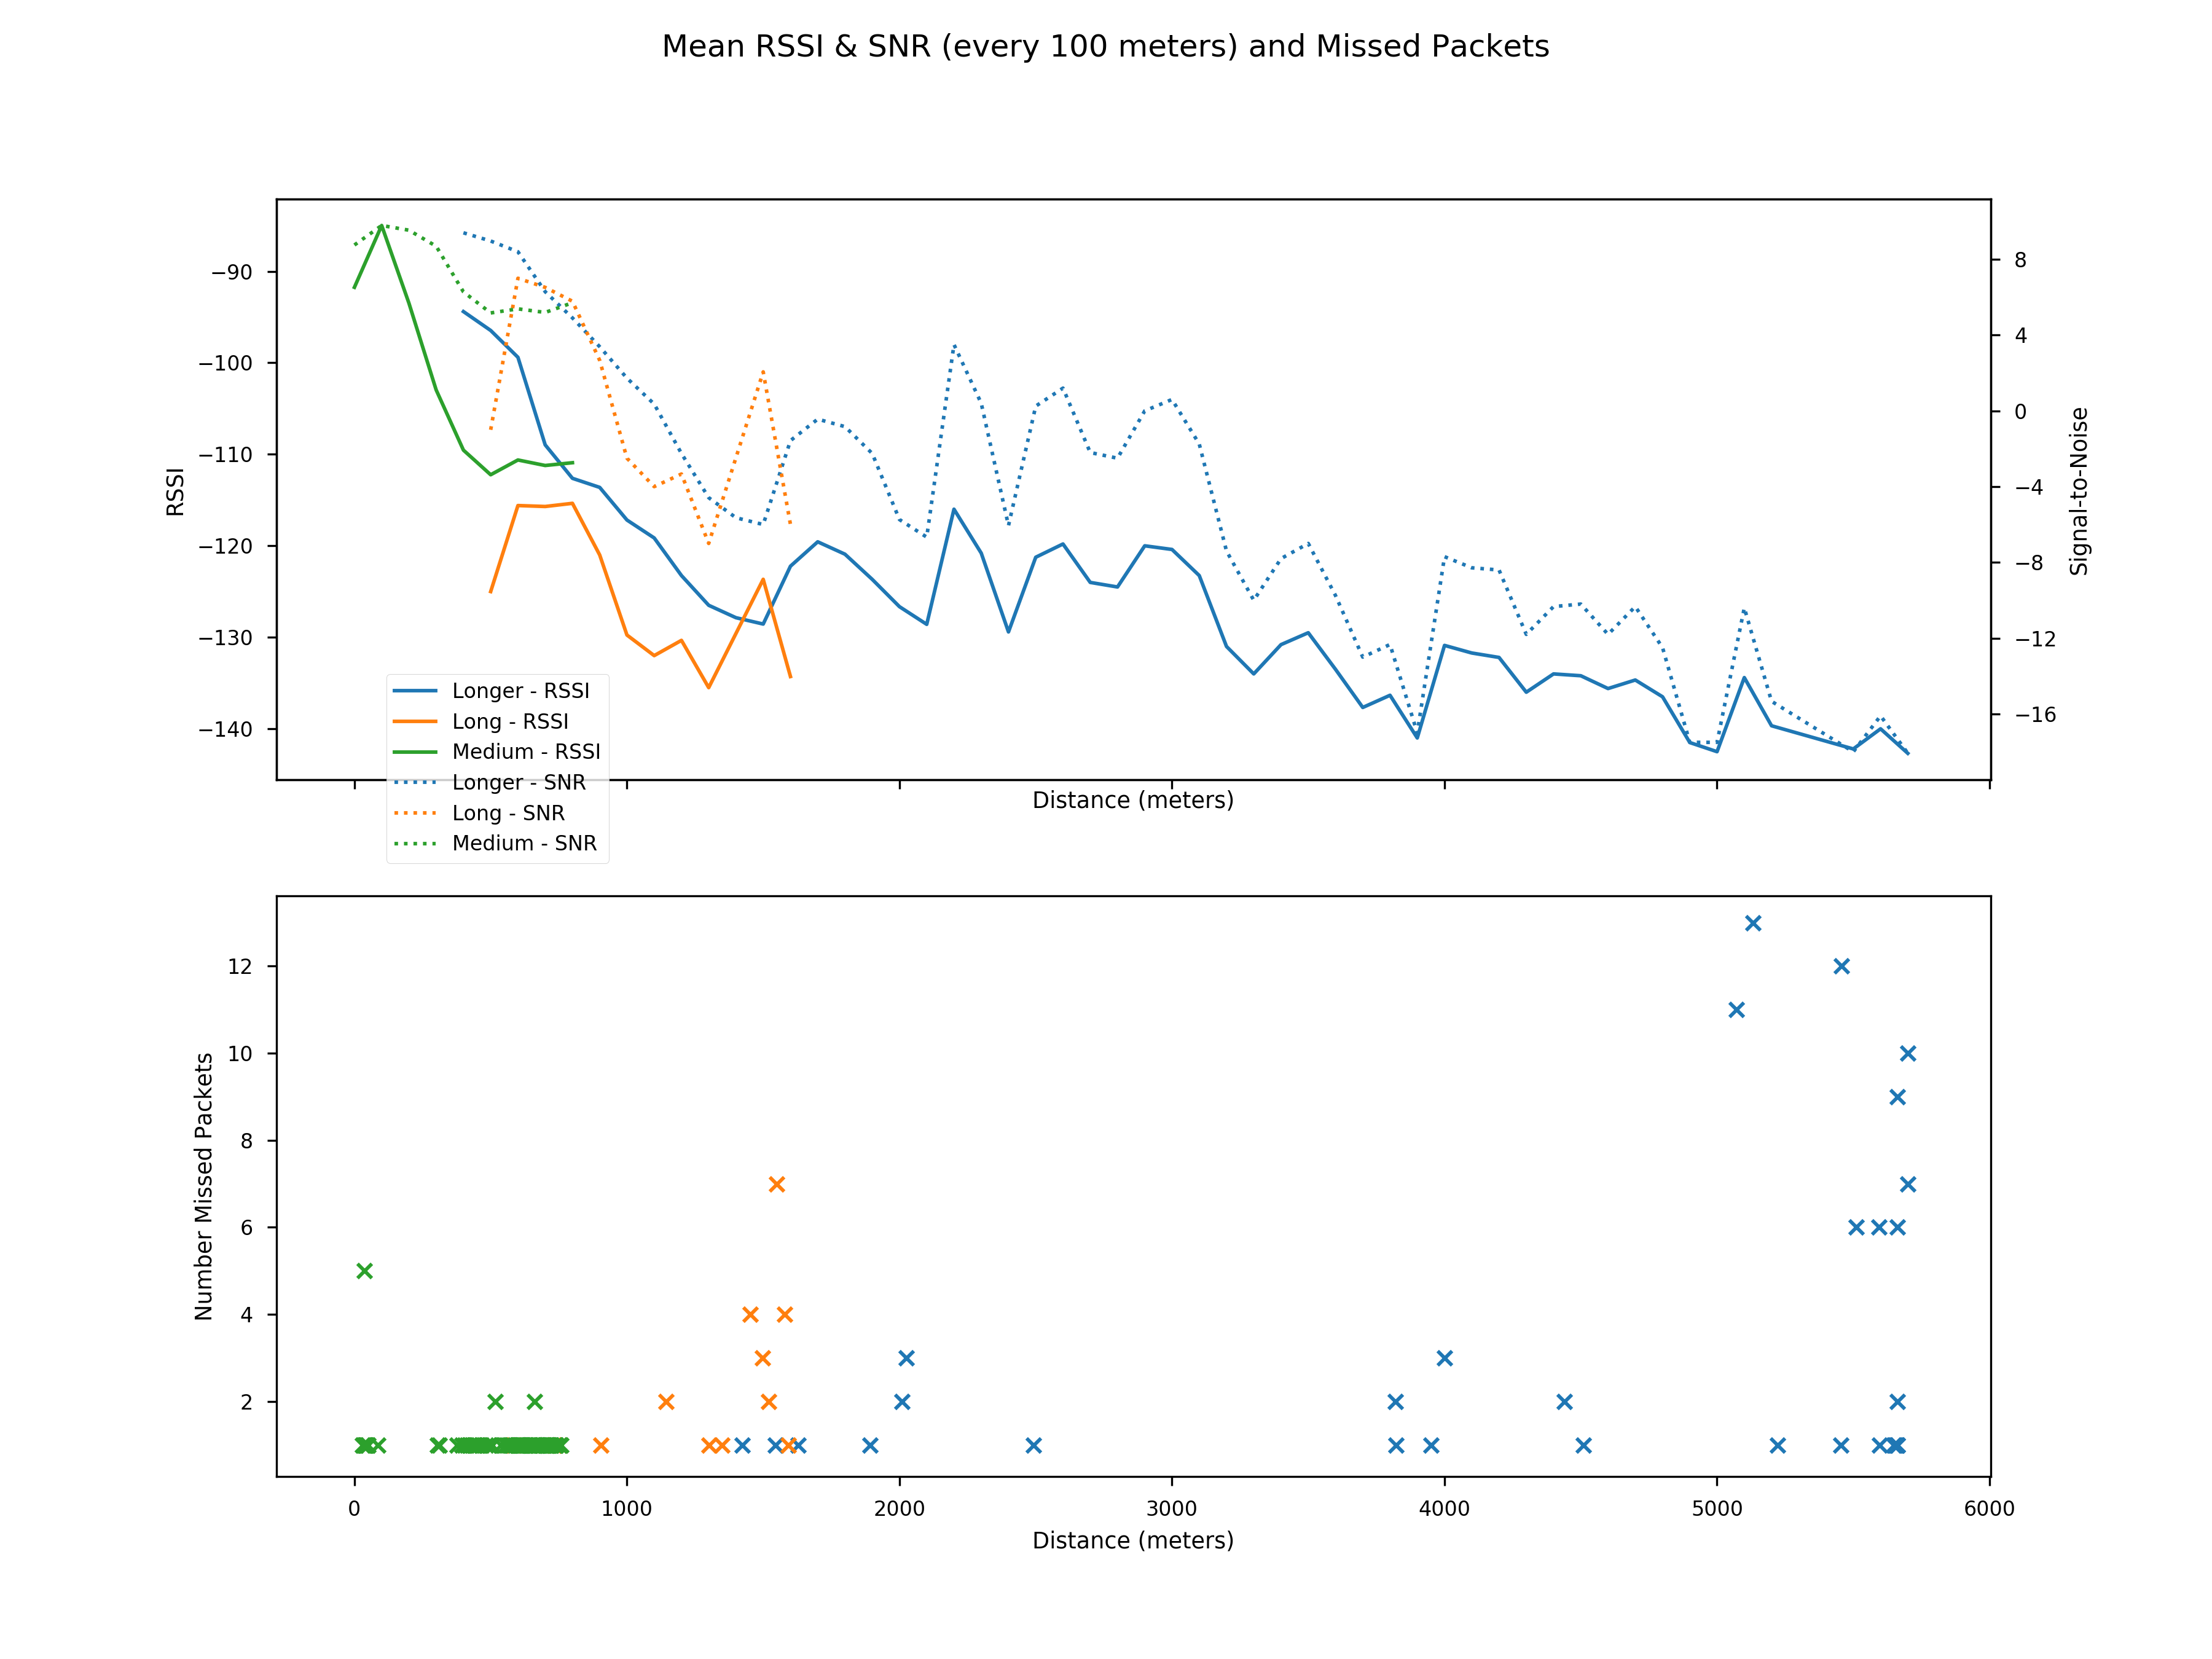
\includegraphics[width=\linewidth]{../img/processed_RSSI_SNR_Missed.png}
\caption{(upper) Mean RSSI \& SNR every 100 meters and (lower) Missed Packets}
\label{results-chart}
\end{center}
\end{figure*}

\section{Waterfall Visualization}
Most SDR software has a waterfall visualization component. It is a graph overtime (axis 1) of the frequency's (axis 2) amplitude (axis 3, usually color intensity). High spreading factor chirps can very easily be seen when it is updating fast enough. Figure \ref{fig:waterfall-compare} shows a similar transmission received from far away and near by. The ability to view the waterfall of a signal gave the ability to check that the a signal was actually being received at the desired frequency and bandwidth when first starting analysis. Due to limitations in the SDR used and computer processors speed, only the transmissions with spreading factor of 12 could resolve individual chirps live using the CubicSDR software. Other smaller spreading factor settings were nonetheless obvious from the water fall as their power dominated the band. The other spreading factors were still able to be resolved to chirps by throttling a raw ``IQ" file after recording it with a small GNU Radio flow graph (discussed later in section \ref{sec:gr-record}, figure \ref{fig:rtl-gr-recorder}).

\section{LoRa PHY Encoding and Modulation}
\label{sec:EncAndMod}

Much of the summarized information in this section was discovered experientially or otherwise by M. Knight and the Bastille Threat Research Team (Bastille)\cite{grcon}. An understanding of how official LoRa radios encode and modulate data is essential to decoding the raw signal and realizing its long range ability.

\subsection{De-chirping}
A symbol is represented as a instant change in frequency of a chirp back to the lower frequency. By multiplying a symbolic chirp by a locally generated opposite chirp and taking a $2^{spreading factor}$ bin Fast Fourier Transform(FFT), the bin index with the greatest amplitude contains the encoded symbol. This is \textit{not a bit or byte}, next it must be decoded.

\subsection{Preamble and Start of Frame}
The preamble (a number of continuous up-chirps) and start of frame delimiter (two down-chirps) indicate the start of a data frame. After being de-chirped, consecutive FFT bins with the same symbol indicate the preamble. The two synchronization down-chirps are de-chirped similarly using overlapping FFTs to improve temporal resolution for synchronization (since it is more computationally expensive).

\subsection{Whitening and Interleaving}
Data whitening purposely introduces randomness into the symbols for other features (like clock recovery) that would be implemented by a receiver. True symbols are extracted with an XOR operation. \texttt{gr-lora} experimentally determined the whitening sequence by transmitting zeros.

Interleaving scrambles bits to make received data stronger against bursts of interference. Knight claims that the interleaver described in a patent filing is not implemented by the standard and concluded that it uses a type of diagonal interleaver\cite{grcon}.

\subsection{Forward Error Correction}
LoRa uses Hamming codes as a means to correct bits flipped in transit by adding redundancy to the transmission. LoRa uses a fractional representation: 

\begin{equation}
\frac{\# data bits}{\# data bits + \# parity bits}
\end{equation}
\ %br

For example: 4/5; a total of 5 bits encodes 4 data bits. See the `Hamming' column in Table \ref{tab:tested-settings} for some used by the RadioHead library for LoRa capable radios. LoRa has the bits in nonstandard order that must be adjusted before fully decoding. The result of applying forward error correction is the actual data of the PHY packet.

\section{Software Defined Radio}
A software defined radio (SDR) abstracts radio circuity to be implemented by software instead. The hardware component is an analog to digital converter. This makes SDRs incredibly flexible -- especially when dealing with scanning local frequencies and doing custom signal processing on them. For this project, an inexpensive RTL-SDR\footnote{SDR Model: R820T2 RTL2832U 1PPM TCXO SMA V3 Dongle} dongle was used.

\section{Decoding with SDR}

\subsection{GNU Radio}
GNU Radio\cite{gnuradio} is a free(libre) software tool for interfacing with SDRs and performing signal processing on the input. It comes with many ``blocks" of processing that are connected together to form a ``flowgraph". Example blocks include: FM (De)modulation, low pass filter, FFT, WAV file sink, and GUI waterfall sink. These flowgraphs are `compiled' to a Python script to be run. Custom blocks can be written in Python or C++ (as a class) an integrated into a flowgraph. In this project GNU Radio is used to perform the actual decoding of LoRa packets in a frequency flexible way. GNU Radio was installed on a Debian machine for this project.

As mentioned previously, SDR allows the recoding of raw ``IQ" signals for later processing. This is a technique used for feeding signals into GNU Radio that are attempting to be decoded. It makes it simple to pre-record various transmissions with the ability to later switch between and throttle them (making it easier on the processor).

\subsection{Recording IQ Files}
\label{sec:gr-record}
To make decoding attempts easier to perform, raw IQ (In-phase/quadrature) signals were recorded using a simple GNU Radio flowgraph (figure \ref{fig:rtl-gr-recorder}). IQ signals are a means of digitally storing samples of radio data as two amplitude modulated sinusoids without the loss of information. These files are later used as a source for demodulating and decoding flowgraph (figure \ref{fig:gr-decode-graph}).

% GR Recorder graph
\begin{figure}[htbp]
\begin{center}
\includegraphics[width=7cm]{../img/RTL-gr-recorder-graph.png}
\caption{The left RTL `source' block pipes the data into an output file (sink) and a live GUI waterfall.}
\label{fig:rtl-gr-recorder}
\end{center}
\end{figure}

\subsection{\texttt{gr-lora} out of tree (OOT) module}
\texttt{gr-lora} is an OOT module for GNU Radio. It is a (limited) open source implementation of LoRa based on blind signal analysis by Matt Knight and Bastille. It is used as a stepping off point for this paper.


\begin{figure*}[]
\begin{center}
\includegraphics[width=15cm]{../img/success1-GR-decode-graph.png}
\caption{Flowgraph used to decode LoRa signals. The `variable' blocks are used to match signal parameters.}
\label{fig:gr-decode-graph}
\end{center}
\end{figure*}

\subsection{Switching Transmitter Library}
After multiple failed attempts to demodulate a signal using gr-lora (before even decoding), reading past issues on GitHub lead to the discovery that gr-lora only supports ``implicit header" mode -- the whitening sequences are different. Since RadioHead only supports ``explicit header" mode, the Arduino based transmitter software was switched\footnote{RadioHead was originally used due to its general popularity, greater chip support, the fact that sending a packet does not block code execution, and unawareness of the arduino-LoRa library at the time.} to use Sandeep Mistry's ``Arduino LoRa" library\cite{sandeep}. It allows more control of the LoRa header, spreading factor, bandwidth, and hamming code rate. Using this library, something like the following can be setup (full code in appendix):

\begin{Verbatim}

LoRa.setSpreadingFactor(7);
LoRa.setSignalBandwidth(125E3);
LoRa.setCodingRate4(5); // 4/5

// ...

LoRa.beginPacket(true); // implicit header
uint8_t pkt[] = {0x12,0x34,0x56,0x78,0x9a};
LoRa.write(pkt, 5);
LoRa.endPacket(); // block & transmit
\end{Verbatim}


\subsection{Decoding Flowgraph}
Figure \ref{fig:gr-decode-graph} displays the GNU Radio flowgraph used to successfully demodulate and decode LoRa PHY signals. The design is based on examples provided by gr-lora. Two blocks handle the \textit{demodulating} and \textit{decoding} individually (chirps to symbols and symbols to bytes, respectively). It did not always decode perfectly, at times a few bits were incorrect. From online discussion, the issue seems to come from the de-interleaver not being ideal. The major of decoding is correct.

\section{Importance of physical layer security}

The physical layer is the fundamental component of all communication systems. The wireless physical layer is exposed to the world by its very nature -- it is ubiquitous and vulnerable. No matter encryption, a simple spectrogram will show if and when a communication is occurring in some radius around the evesdropper. As the number of wireless devices and sensors increases, so does the attack surface. Therefore securing this layer is important to securing the rest of the stack for commercial, military, scientific, emergency, and human rights usage. 

\subsection{Packet in Packet}

The proclaimed ``Packet in Packet" attack\cite{pkt-in-pkt} is a method for indiscriminately embedding physical layer data frames via upper layer protocols by abusing standard compliant preambles and error correction. This method can avoid intrusion detection systems and firewalls. 

Essentially, the entire physical layer packet data is embedded into, say, a link layer frame. When a crafted error occurs on the link layer frame's checksum, the physical layer (and possibly malicious) packet is interpreted instead. The start of frame delimiter in IEEE 802.15.4 (e.g. Zigbee) is simply a specific byte (\texttt{xA7}), so it can be placed in upper layer payloads.

LoRa uses two reverse chirps, a `symbol' that can't exist in upper layers, it is only used to sync a receiver with an incoming signal's data. This is strong resistance against this particular attack. 

\subsection{Device Dialects (vulnerability)}
There are slight (but still standard compliant) implementation differences in some commercial IEEE 802.15.4 radio chips. These `dialects' --as the researchers coined-- allow the transmission of packets that can only be `heard' by specific devices, thus never being received by any other radios. That includes intrusion detection devices on a wireless network.\cite{dialect}

\subsection{Jamming}
Radio jamming is one of the simplest and effective techniques of preventing availability. It is the physical layer equivalent of denial of service. LoRa is susceptible to selective jamming where ``a malicious jammer can systematically jam either a particular type of message or all messages coming from a particular end-device." \cite{lora-jam}

There are two methods that change the spreading factor to resist this attack: (1) Use a large spreading factor --like 12-- to "beat" the jammer RSSI and (2) reduce an attacker's reaction time by using a small spreading factor, thus being ``in the air" for a shorter duration.

\section{Further Work}
As it developed, this research and paper became a combination survey-experimentation of LoRa knowledge. Scanning a range of frequencies for a LoRa signal (and attempting to determine its parameters like spreading factor and bandwidth) may be an interesting next step, but a more difficult undertaking. The implementation of more PHY features (such as explicit header whitening and clock recovery) in OOT modules, like gr-lora, should also be continued. Further improving the physical layer and implementing the LoRa WAN (link layer) would be interesting future investigations. 

Continuing to investigate packet in packet, potential device dialects, and any other security vulnerabilities would obviously also be important work.

\section{Concepts Learned}
I have been wanting to experiement with SDRs for some time. This project gave me the nudge to get started. Thusly, I learned the basics of SDRs, how they work, and how they interact with radio waves. The ability to visualize and `play' with signals also gave me a much greater intuition of the radio spectrum.

This ability came from the GUI listening software (e.g. CubicSDR, GQRX) and GNU Radio. I also learned the basics of GNU Radio, its patterns, the functions of different blocks, and how wiggling one thing affects another.

I also learned a lot about physical layer protocols in general -- partly from a visual intuition perspective with spectrograms and partly from a mathematical one with IQ and (de)modulation. Of course, I also learned (in more detail) how LoRa PHY works, and what it is capable of.

\section{Conclusion}
This project demonstrated the range and data speed of inexpensive low power LoRa radios. It also (after several failed attempts) worked to understand and decode signals from an official transceiver using an inexpensive SDR dongle and GNU Radio. The physical layer attack surface is ever growing -- it is important to understand and secure it.

\newpage % shift to next column to even out

\section{Acknowledgments}
The idea of this project came from my participation in FL Polytechnics's ASTRO Rocket Design club. I have been working on a long distance (at least 3000 meters) payload telemetry system. I started programming for these LoRa modules purchased by the club in the previous semester. We are using the same two-radio reception system described in section 3 (Range Testing). I thought it would be nice to also have a more extensible model for potential future use (multiple receivers with different antennas for redundancy). I combined these goals into this project.

Additionally, Matt Knight's research and conference talks were a great starting point for this project.

%%%%%%%%%%%%%%%%%%%%%%%%%%%%%%%%%%%%%%%%%%%

\bibliographystyle{IEEEtran} % unsrt
\bibliography{refs}

\clearpage
\section*{Appendix}
%\appendix
\section{Appendix A: The OpenFlow Protocol}
The heart of the OpenFlow spec is the set of structures used for OpenFlow Protocol messages.  
\\\\
The structures, defines, and enumerations described below are derived from the file \verb|include/openflow/openflow.h|, which is part of the standard OpenFlow distribution.  All structures are packed with padding and 8-byte aligned, as checked by the assertion statements.  All OpenFlow messages are sent in big-endian format.  

\subsection{OpenFlow Header}
Each OpenFlow message begins with the OpenFlow header:

\input{struct/ofp_header}
The version specifies the OpenFlow protocol version being used.  During the current draft phase of the OpenFlow Protocol, the most significant bit will be set to indicate an experimental version and the lower bits will indicate a revision number.  The current version is \input{define/OFP_VERSION}.  The final version for a Type 0 switch will be 0x00.  The length field indicates the total length of the message, so no additional framing is used to distinguish one frame from the next.  The type can have the following values:

\input{enum/ofp_type}

\subsection{Common Structures}
This section describes structures used by multiple messages.

\subsubsection{Port Structures}
Physical ports are described with the following structure:

\input{struct/ofp_phy_port}
The \verb|port_no| field is a value the datapath associates with a physical port.  The \verb|hw_addr| field typically is the MAC address for the port; \verb|OFP_MAX_ETH_ALEN| is 6.  The name field is a null-terminated string containing a human-readable name for the interface.  The value of \verb|OFP_MAX_PORT_NAME_LEN| is 16.  
\\\\
The \verb|config| field describes spanning tree and administrative settings with the following structure:

\input{enum/ofp_port_config}
The port config bits indicate whether a port has been administratively brought down, options for handling 802.1D spanning tree packets, and how to handle incoming and outgoing packets.   These bits, configured over multiple switches, enable an OpenFlow network to safely flood packets along either a custom or 802.1D spanning tree.
\\\\
The controller may set \verb|OFPPFL_NO_STP| to 0 to enable STP on a port or to 1 to disable STP on a port. (The latter corresponds to the Disabled STP port state.) The default is switch implementation-defined; the OpenFlow reference implementation by default sets this bit to 0 (enabling STP).
\\\\
When \verb|OFPPFL_NO_STP| is 0, STP controls the \verb|OFPPFL_NO_FLOOD| and \verb|OFPPFL_STP_*| bits directly. \verb|OFPPFL_NO_FLOOD| is set to 0 when the STP port state is Forwarding, otherwise to 1. The bits in \verb|OFPPFL_STP_MASK| are set to one of the other \verb|OFPPFL_STP_*| values according to the current STP port state.
\\\\
When the port flags are changed by STP, the switch sends an \verb|OFPT_PORT_STATUS| message to notify the controller of the change. The \verb|OFPPFL_NO_RECV|, \verb|OFPPFL_NO_RECV_STP|, \verb|OFPPFL_NO_FWD|, and \verb|OFPPFL_NO_PACKET_IN| bits in the OpenFlow port flags may be useful for the controller to implement STP, although they interact poorly with in-band control. 
\\\\
The \verb|state| field describes the spanning tree state and whether a physical link is present, with the following structure:

\input{enum/ofp_port_state}
All port state bits are read-only, representing spanning tree and physical link state.
\\\\
The port numbers use the following conventions:

\input{enum/ofp_port}
The \verb|curr|, \verb|advertised|, \verb|supported|, and \verb|peer| fields indicate link modes (10M to 10G full and half-duplex), link type (copper/fiber) and link features (autonegotiation and pause).  Port features are represent by the following structure:

\input{enum/ofp_port_features}
Multiple of these flags may be set simultaneously.

\subsubsection{\qosupd{Queue Structures}}
\label{cts:qos}
\qosupd{An OpenFlow switch provides limited Quality-of-Service support
  (QoS) through a simple queuing
mechanism. One (or more) queues can attach to a port and be used to map flows
on it. Flows mapped to a specific queue will be treated according to
that queue's configuration (e.g. min rate).
\\\\
A queue is described by the} \verb|ofp_packet_queue| \qosupd{structure:
\input{struct/ofp_packet_queue}
Each queue is further described by a set of properties, each of a
specific type and configuration.
\input{enum/ofp_queue_properties}
Each queue property description starts with a common header:
\input{struct/ofp_queue_prop_header}
Currently, there is only a minimum-rate type queue, described by the}
\verb|ofp_queue_prop_min_rate| \qosupd{structure:
\input{struct/ofp_queue_prop_min_rate}}

\subsubsection{Flow Match Structures}
When describing a flow entry, the following structure is used:

\input{struct/ofp_match}
The \verb|wildcards| field has a number of flags that may be set:

\input{enum/ofp_flow_wildcards}
If no wildcards are set, then the \verb|ofp_match| exactly describes a flow, over the entire OpenFlow 12-tuple.  On the other extreme, if all the wildcard flags are set, then every flow will match.
\\\\
The source and destination netmasks are each specified with a 6-bit number in the wildcard description. It is interpreted similar to the CIDR suffix, but with the opposite meaning, since this is being used to indicate which bits in the IP address should be treated as ``wild". For example, a CIDR suffix of "24" means to use a netmask of ``255.255.255.0". However, a wildcard mask value of ``24" means that the least-significant 24-bits are wild, so it forms a netmask of ``255.0.0.0". 

\subsubsection{Flow Action Structures}
A number of actions may be associated with flows or packets.  The currently defined action types are:

\input{enum/ofp_action_type} 
Output \qosupd{and enqueue} actions are described in Section \ref{ft:actions}, while Field-Modify actions are described in Table \ref{table:field modify actions}.  An action definition contains the action type, length, and any associated data:

\input{struct/ofp_action_header}
An \verb|action_output| has the following fields:

\input{struct/ofp_action_output}
The \verb|max_len| indicates the maximum amount of data from a packet that should be sent when the port is \verb|OFPP_CONTROLLER|.  If \verb|max_len| is zero, the switch must send a zero-size \verb|packet_in| message.  The \verb|port| specifies the physical port from which packets should be sent. 
 \\\\
\qosupd{The enqueue action maps a flow to an already-configured queue, regardless of the TOS and VLAN PCP bits.
  The packet should not change after an enqueue action. If the switch
  needs to set the TOS/PCP bits for internal handling, the original values
  should be restored before sending the packet out.
\\\\
A switch may support only queues that are tied to specific PCP/TOS
bits. In that case, we cannot map an arbitrary flow to a specific
queue, therefore the action ENQUEUE is not supported. The user can
still use these queues and map
flows to them by setting the relevant fields (TOS, VLAN PCP).
\\\\
The enqueue action has the following fields:

\input{struct/ofp_action_enqueue}}
An \verb|action_vlan_vid| has the following fields:

\input{struct/ofp_action_vlan_vid}
The \verb|vlan_vid| field is 16 bits long, when an actual VLAN id is only 12 bits. The value \verb|0xffff| is used to indicate that no VLAN id was set.
\\\\
An \verb|action_vlan_pcp| has the following fields:

\input{struct/ofp_action_vlan_pcp}
The \verb|vlan_pcp| field is 8 bits long, but only the lower 3 bits have meaning.  
\\\\
An \verb|action_strip_vlan| takes no arguments and consists only of a generic \verb|ofp_action_header|.  This action strips the VLAN tag if one is present.
\\\\
An \verb|action_dl_addr| has the following fields:

\input{struct/ofp_action_dl_addr}
The \verb|dl_addr| field is the MAC address to set.
\\\\
An \verb|action_nw_addr| has the following fields:

\input{struct/ofp_action_nw_addr}
The \verb|nw_addr| field is the IP address to set.
\\\\
An \verb|action_nw_tos| has the following fields:

\input{struct/ofp_action_nw_tos}
The \verb|nw_tos| field is the 6 upper bits of the ToS field to set, in the original bit positions (shifted to the left by 2).
\\\\
An \verb|action_tp_port| has the following fields:

\input{struct/ofp_action_tp_port}
The \verb|tp_port| field is the TCP/UDP/other port to set.
\\\\
An \verb|action_vendor| has the following fields:

\input{struct/ofp_action_vendor_header}
The \verb|vendor| field is the Vendor ID, which takes the same form as in struct \verb|ofp_vendor|.

\subsection{Controller-to-Switch Messages}

\subsubsection{Handshake}
\label{cts:handshake} 
Upon TLS session establishment, the controller sends an \verb|OFPT_FEATURES_REQUEST| message.  This message does not contain a body beyond the OpenFlow header.  The switch responds with an \verb|OFPT_FEATURES_REPLY| message:

\input{struct/ofp_switch_features}
The \verb|datapath_id| field uniquely identifies a datapath.  The lower 48 bits are intended for the switch MAC address, while the top 16 bits are up to the implementer.  An example use of the top 16 bits would be a VLAN ID to distinguish multiple virtual switch instances on a single physical switch.  This field should be treated as an opaque bit string by controllers.
\\\\
The \verb|n_tables| field describes the number of tables supported by the switch, each of which can have a different set of supported wildcard bits and number of entries.  When the controller and switch first communicate, the controller will find out how many tables the switch supports from the Features Reply. If it wishes to understand the size, types, and order in which tables are consulted, the controller sends a \verb|OFPST_TABLE| stats request. A switch must return these tables in the order the packets traverse the tables, with all exact-match tables listed before all tables with wildcards.
\\\\
The \verb|capabilities| field uses the following flags:

\input{enum/ofp_capabilities} 
The \verb|actions| field is a bitmap of actions supported by the switch.  The list of actions is found in Section~\ref{ft:actions}; all actions marked Required must be supported. Vendor actions should \emph{not} be reported via this bitmask. The bitmask uses the values from \verb|ofp_action_type| as the number of bits to shift left for an associated action. For example, \verb|OFPAT_SET_DL_VLAN| would use the flag \verb|0x00000002|.
\\\\
The \verb|ports| field is an array of \verb|ofp_phy_port| structures that describe all the physical ports in the system that support OpenFlow.  The number of port elements is inferred from the length field in the OpenFlow header. 

\subsubsection{Switch Configuration}
The controller is able to set and query configuration parameters in the switch with the \verb|OFPT_SET_CONFIG| and \verb|OFPT_GET_CONFIG_REQUEST| messages, respectively.  The switch responds to a configuration request with an \verb|OFPT_GET_CONFIG_REPLY| message; it does not reply to a request to set the configuration.  
\\\\
There is no body for \verb|OFPT_GET_CONFIG_REQUEST| beyond the OpenFlow header.  The \verb|OFPT_SET_CONFIG| and \verb|OFPT_GET_CONFIG_REPLY| use the following:

\input{struct/ofp_switch_config}
The configuration flags include the following:

\input{enum/ofp_config_flags}
The \verb|OFPC_FRAG_*| flags indicate whether IP fragments should be treated normally, dropped, or reassembled.  ``Normal" handling of fragments means that an attempt should be made to pass the fragments through the OpenFlow tables. If any field is not present (e.g., the TCP/UDP ports didn't fit), then the packet should not match any entry that has that field set.
\\\\
The \verb|miss_send_len| field defines the number of bytes of each packet sent to the controller as a result of both flow table misses and flow table hits with the controller as the destination.  If this field equals 0, the switch must send a zero-size \verb|packet_in| message.

\subsubsection{Modify State Messages}
\paragraph{Modify Flow Entry Message}
Modifications to the flow table from the controller are done with the \verb|OFPT_FLOW_MOD| message:

\input{struct/ofp_flow_mod}
The \verb|cookie| field is an opaque data value that is set by the
controller.  It is not used in any matching functions, and thus does not
need to reside in hardware.  The value -1 (0xffffffffffffffff) is
reserved and must not be used.  It is required that when \verb|command| is
\verb|OFPC_MODIFY| or \verb|OFPC_MODIFY_STRICT| that matched flows have
their \verb|cookie| field updated appropriately.
\\\\
The \verb|command| field must be one of the following:

\input{enum/ofp_flow_mod_command}
The differences between \verb|OFPFC_MODIFY| and \verb|OFPFC_MODIFY_STRICT| are explained in Section \ref{flow_table:sec_chan:flow_mod} and differences between \verb|OFPFC_DELETE| and \verb|OFPFC_DELETE_STRICT| are explained in Section \ref{flow_table:sec_chan:flow_removal}. 
\\\\
The \verb|idle_timeout| and \verb|hard_timeout| fields control how quickly flows expire.  
\\\\
If the \verb|idle_timeout| is set and the \verb|hard_timeout| is zero, the entry must expire after \verb|idle_timeout| seconds with no received traffic.  If the \verb|idle_timeout| is zero and the \verb|hard_timeout| is set, the entry must expire in \verb|hard_timeout| seconds regardless of whether or not packets are hitting the entry.
\\\\
If both \verb|idle_timeout| and \verb|hard_timeout| are set, the flow will timeout after \verb|idle_timeout| seconds with no traffic, or \verb|hard_timeout| seconds, whichever comes first.  If both \verb|idle_timeout| and \verb|hard_timeout| are zero, the entry is considered permanent and will never time out.  It can still be removed with a \verb|flow_mod| message of type \verb|OFPFC_DELETE|. 
\\\\
The \verb|priority| field is only relevant for flow entries with wildcard fields.  The priority field indicates table priority, where higher numbers are higher priorities; the switch must keep the highest-priority wildcard entries in the lowest-numbered (fastest) wildcard table, to ensure correctness.  It is the responsibility of each switch implementer to ensure that exact entries always match before wildcards entries, regardless of the table configuration.  
\\\\
The \verb|buffer_id| refers to a buffered packet sent by the \verb|OFPT_PACKET_IN| message.
\\\\
The \verb|out_port| field optionally filters the scope of DELETE and DELETE\_STRICT messages by output port.  If \verb|out_port| contains a value other than \verb|OFPP_NONE|, it introduces a constraint when matching.  This constraint is that the rule must contain an output action directed at that port.  Other constraints such as \verb|ofp_match| structs and priorities are still used; this is purely an \emph{additional} constraint.  Note that to disable output port filtering, \verb|out_port| must be set to \verb|OFPP_NONE|, since 0 is a valid port id.  This field is ignored by ADD, MODIFY, and MODIFY\_STRICT messages.
\\\\
The \verb|flags| field may include the follow flags:

\input{enum/ofp_flow_mod_flags}
When the \verb|OFPFF_SEND_FLOW_REM| flag is set, the switch must send a flow removed message when the flow expires.  The default is for the switch to not send flow removed messages for newly added flows.  
\\\\
When the \verb|OFPFF_CHECK_OVERLAP| flag is set, the switch must check that there are no conflicting entries with the same priority. If there is one, the flow mod fails and an error code is returned.
\\\\
When the \verb|OFPFF_EMERG_| flag is set, the switch must consider this flow entry as an emergency entry, and only use it for forwarding when disconnected from the controller.

\paragraph{Port Modification Message}
The controller uses the \verb|OFPT_PORT_MOD| message to modify the behavior of the physical port:

\input{struct/ofp_port_mod}
The \verb|mask| field is used to select bits in the \verb|config| field to change.  The \verb|advertise| field has no mask; all port features change together.

\subsubsection{\qosupd{Queue Configuration Messages}}
\qosupd{Queue configuration takes place outside the OpenFlow protocol, either
  through a command line tool or through an external dedicated configuration
protocol.
\\\\
The controller can query the switch for configured queues on a port
using the following structure:
\input{struct/ofp_queue_get_config_request}
The switch replies back with an} \verb|ofp_queue_get_config_reply| \qosupd{command, containing
a list of configured queues.

\input{struct/ofp_queue_get_config_reply}
}

\subsubsection{Read State Messages}
While the system is running, the datapath may be queried about its current state using the \verb|OFPT_STATS_REQUEST| message:

\input{struct/ofp_stats_request}
The switch responds with one or more \verb|OFPT_STATS_REPLY| messages:

\input{struct/ofp_stats_reply}
The only value defined for \verb|flags| in a reply is whether more replies will follow this one - this has the value \verb|0x0001|.  To ease implementation, the switch is allowed to send replies with no additional entries.  However, it must always send another reply following a message with the �more� flag set.  The transaction ids (xid) of replies must always match the request that prompted them.
\\\\
In both the request and response, the \verb|type| field specifies the kind of information being passed and determines how the \verb|body| field is interpreted:

\input{enum/ofp_stats_types}

\paragraph{Description Statistics}
Information about the switch manufacturer, hardware revision, software revision, serial number, and a description field is available from the \verb|OFPST_DESC| stats request type:

\input{struct/ofp_desc_stats}
Each entry is ASCII formatted and padded on the right with null bytes (\textbackslash0).  \verb|DESC_STR_LEN| is \input{define/DESC_STR_LEN}and \verb|SERIAL_NUM_LEN| is \input{define/SERIAL_NUM_LEN}.  Note: \footnote{Added to address concerns raised in \url{https://mailman.stanford.edu/pipermail/openflow-spec/2009-September/000504.html}} the \verb|dp_desc| field is a free-form string to describe the datapath for debugging purposes, e.g., ``switch3 in room 3120''.  As such, it is not guaranteed to be unique and should not be used as the primary identifier for the datapath---use the \verb|datapath_id| field from the switch features instead (\S~\ref{cts:handshake}).

\paragraph{Individual Flow Statistics}
Information about individual flows is requested with the \verb|OFPST_FLOW| stats request type:

\input{struct/ofp_flow_stats_request}
The \verb|match| field contains a description of the flows that should be matched and may contain wildcards.  This field's matching behavior is described in Section \ref{flow_table:sec_chan:flow_add}.
\\\\
The \verb|table_id| field indicates the index of a single table to read, or \verb|0xff| for all tables.
\\\\
The \verb|out_port| field optionally filters by output port.  If \verb|out_port| contains a value other than \verb|OFPP_NONE|, it introduces a constraint when matching.  This constraint is that the rule must contain an output action directed at that port.  Other constraints such as \verb|ofp_match| structs are still used; this is purely an \emph{additional} constraint.  Note that to disable output port filtering, \verb|out_port| must be set to \verb|OFPP_NONE|, since 0 is a valid port id. 
\\\\
The \verb|body| of the reply consists of an array of the following:

\input{struct/ofp_flow_stats}
The fields consist of those provided in the \verb|flow_mod| that created these, plus the table into which the entry was inserted, the packet count, and the byte count.
\\\\
\label{flow_duration_info}The \verb|duration_sec| and \verb|duration_nsec| fields indicate the elapsed time the flow has been installed in the switch. The total duration in nanoseconds can be computed as $\verb|duration_sec|*10^{9}$ + \verb|duration_nsec|. Implementations are required to provide millisecond precision; higher precision is encouraged where available.

\paragraph{Aggregate Flow Statistics}
Aggregate information about multiple flows is requested with the \verb|OFPST_AGGREGATE| stats request type:

\input{struct/ofp_aggregate_stats_request}
The \verb|match| field contains a description of the flows that should be matched and may contain wildcards.  This field's matching behavior is described in Section \ref{flow_table:sec_chan:flow_add}.
\\\\
The \verb|table_id| field indicates the index of a single table to read, or \verb|0xff| for all tables.
\\\\
The \verb|out_port| field optionally filters by output port.  If \verb|out_port| contains a value other than \verb|OFPP_NONE|, it introduces a constraint when matching.  This constraint is that the rule must contain an output action directed at that port.  Other constraints such as \verb|ofp_match| structs are still used; this is purely an \emph{additional} constraint.  Note that to disable output port filtering, \verb|out_port| must be set to \verb|OFPP_NONE|, since 0 is a valid port id. 
\\\\
The \verb|body| of the reply consists of the following:

\input{struct/ofp_aggregate_stats_reply} 

\paragraph{Table Statistics}
Information about tables is requested with the \verb|OFPST_TABLE| stats request type.  The request does not contain any data in the body.
\\\\
The body of the reply consists of an array of the following:

\input{struct/ofp_table_stats}
The \verb|body| contains a \verb|wildcards| field, which indicates the fields for which that particular table supports wildcarding. For example, a direct look-up hash table would have that field set to zero, while a sequentially searched table would have it set to \verb|OFPFW_ALL|. The entries are returned in the order that packets traverse the tables. 
\\\\
\verb|OFP_MAX_TABLE_NAME_LEN| is \input{define/OFP_MAX_TABLE_NAME_LEN}.

\paragraph{Port Statistics}
Information about physical ports is requested with the \verb|OFPST_PORT| stats request type:

\input{struct/ofp_port_stats_request}
The \verb|port_no| field optionally filters the stats request to the given port.  To request all port statistics, \verb|port_no| must be set to \verb|OFPP_NONE|.
\\\\
The \verb|body| of the reply consists of an array of the following:

\input{struct/ofp_port_stats}
The switch should return a value of -1 for unavailable counters.

\paragraph{\qosupd{Queue Statistics}}
\qosupd{The} \verb|OFPST_QUEUE| \qosupd{stats request message provides
  queue statistics for one or more ports.
  The request body consists of a} \verb|port_no| \qosupd{field
identifying the port and a} \verb|queue_id|. \verb|OFPP_ALL|
\qosupd{refers to all ports, while} \verb|OFPQ_ALL| \qosupd{refers to all queues configured
at a port.

\input{struct/ofp_queue_stats_request}
The body of the reply consists of an array of
the following structure:

\input{struct/ofp_queue_stats}}

\paragraph{Vendor Statistics}
Vendor-specific stats messages are requested with the \verb|OFPST_VENDOR| stats type. The first four bytes of the message are the vendor identifier. The rest of the body is vendor-defined.
\\\\
The \verb|vendor| field is a 32-bit value that uniquely identifies the vendor. If the most significant byte is zero, the next three bytes are the vendor's IEEE OUI. If vendor does not have (or wish to use) their OUI, they should contact the OpenFlow consortium to obtain one. 

\subsubsection{Send Packet Message}
When the controller wishes to send a packet out through the datapath, it uses the \verb|OFPT_PACKET_OUT| message:

\input{struct/ofp_packet_out}
The \verb|buffer_id| is the same given in the \verb|ofp_packet_in| message.  If the \verb|buffer_id| is -1, then the packet data is included in the data array. If \verb|OFPP_TABLE| is specified as the output port of an action, the \verb|in_port| in the \verb|packet_out| message is used in the flow table lookup.

\subsubsection{Barrier Message}
When the controller wants to ensure message dependencies have been met or wants to receive notifications for completed operations, it may use an \verb|OFPT_BARRIER_REQUEST| message.  This message has no body.  Upon receipt, the switch must finish processing all previously-received messages before executing any messages beyond the Barrier Request.  When such processing is complete, the switch must send an \verb|OFPT_BARRIER_REPLY| message with the \verb|xid| of the original request.

\subsection{Asynchronous Messages}
\subsubsection{Packet-In Message}
When packets are received by the datapath and sent to the controller, they use the \verb|OFPT_PACKET_IN| message:

\input{struct/ofp_packet_in}
The \verb|buffer_id| is an opaque value used by the datapath to identify a buffered packet.  When a packet is buffered, some number of bytes from the message will be included in the data portion of the message.  If the packet is sent because of a ``send to controller'' action, then \verb|max_len| bytes from the \verb|action_output| of the flow setup request are sent.  If the packet is sent because of a flow table miss, then at least \verb|miss_send_len| bytes from the \verb|OFPT_SET_CONFIG| message are sent.  The default \verb|miss_send_len| is \input{define/OFP_DEFAULT_MISS_SEND_LEN}bytes.  If the packet is not buffered, the entire packet is included in the data portion, and the \verb|buffer_id| is -1.  
\\\\
Switches that implement buffering are expected to expose, through documentation, both the amount of available buffering, and the length of time before buffers may be reused.  A switch must gracefully handle the case where a buffered \verb|packet_in| message yields no response from the controller.  A switch should prevent a buffer from being reused until it has been handled by the controller, or some amount of time (indicated in documentation) has passed.
\\\\
The reason field can be any of these values:

\input{enum/ofp_packet_in_reason}
 
\subsubsection{Flow Removed Message}
If the controller has requested to be notified when flows time out, the datapath does this with the \verb|OFPT_FLOW_REMOVED| message:

\input{struct/ofp_flow_removed}
The \verb|match|, \verb|cookie|, and \verb|priority| fields are the same as those used in the flow setup request.
\\\\
The \verb|reason| field is one of the following:

\input{enum/ofp_flow_removed_reason}
The \verb|duration_sec| and \verb|duration_nsec| fields are described in Section \ref{flow_duration_info}.
\\\\
The \verb|idle_timeout| field is directly copied from the flow mod that created this entry. 
\\\\
With the above three fields, one can find both the amount of time the flow was active, as well as the amount of time the flow received traffic.
\\\\
The \verb|packet_count| and \verb|byte_count| indicate the number of packets and bytes that were associated with this flow, respectively. 
 
\subsubsection{Port Status Message}
As physical ports are added, modified, and removed from the datapath, the controller needs to be informed with the \verb|OFPT_PORT_STATUS| message:

\input{struct/ofp_port_status}
The \verb|status| can be one of the following values:

\input{enum/ofp_port_reason} 

\subsubsection{Error Message}
There are times that the switch needs to notify the controller of a problem.  This is done with the \verb|OFPT_ERROR_MSG| message: 	

\input{struct/ofp_error_msg}
The \verb|type| value indicates the high-level type of error.  The \verb|code| value is interpreted based on the type.  The \verb|data| is variable length and interpreted based on the \verb|type| and \verb|code|; in most cases this is the message that caused the problem.  
\\\\
Error codes ending in \verb|_EPERM| correspond to a permissions error generated by an entity between a controller and switch, such as an OpenFlow hypervisor. 
\\\\
Currently defined error types are:

\input{enum/ofp_error_type}
For the \verb|OFPET_HELLO_FAILED| error \verb|type|, the following \verb|code|s are currently defined:

\input{enum/ofp_hello_failed_code}
The \verb|data| field contains an ASCII text string that adds detail on why the error occurred.
\\\\
For the \verb|OFPET_BAD_REQUEST| error \verb|type|, the following \verb|code|s are currently defined:

\input{enum/ofp_bad_request_code}
The \verb|data| field contains at least 64 bytes of the failed request.
\\\\
For the \verb|OFPET_BAD_ACTION| error \verb|type|, the following \verb|code|s are currently defined:

\input{enum/ofp_bad_action_code}
The \verb|data| field contains at least 64 bytes of the failed request.
\\\\
For the \verb|OFPET_FLOW_MOD_FAILED| error \verb|type|, the following \verb|code|s are currently defined:

\input{enum/ofp_flow_mod_failed_code}
The \verb|data| field contains at least 64 bytes of the failed request.
\\\\
For the \verb|OFPET_PORT_MOD_FAILED| error \verb|type|, the following \verb|code|s are currently defined:

\input{enum/ofp_port_mod_failed_code}
The \verb|data| field contains at least 64 bytes of the failed request.
\\\\
For the \verb|OFPET_QUEUE_OP_FAILED| error \verb|type|, the following \verb|code|s are currently defined:

\input{enum/ofp_queue_op_failed_code}
The \verb|data| field contains at least 64 bytes of the failed request.
\\\\
If the error message is in response to a specific message from the controller, e.g., \verb|OFPET_BAD_REQUEST|, \verb|OFPET_BAD_ACTION|, or \verb|OFPET_FLOW_MOD_FAILED|, then the \verb|xid| field of the header should match that of the offending message.

\subsection{Symmetric Messages}
\subsubsection{Hello}
The \verb|OFPT_HELLO| message has no body; that is, it consists only of an OpenFlow header. Implementations must be prepared to receive a hello message that includes a body, ignoring its contents, to allow for later extensions. 

\subsubsection{Echo Request}
An Echo Request message consists of an OpenFlow header plus an arbitrary-length data field.  The data field might be a message timestamp to check latency, various lengths to measure bandwidth, or zero-size to verify liveness between the switch and controller.

\subsubsection{Echo Reply}
An Echo Reply message consists of an OpenFlow header plus the unmodified data field of an echo request message.
\\\\
In an OpenFlow protocol implementation divided into multiple layers, the echo request/reply logic should be implemented in the "deepest" practical layer.  For example, in the OpenFlow reference implementation that includes a userspace process that relays to a kernel module, echo request/reply is implemented in the kernel module.  Receiving a correctly formatted echo reply then shows a greater likelihood of correct end-to-end functionality than if the echo request/reply were implemented in the userspace process, as well as providing more accurate end-to-end latency timing.

\subsubsection{Vendor}
The Vendor message is defined as follows:

\input{struct/ofp_vendor_header}
The \verb|vendor| field is a 32-bit value that uniquely identifies the vendor. If the most significant byte is zero, the next three bytes are the vendor's IEEE OUI. If vendor does not have (or wish to use) their OUI, they should contact the OpenFlow consortium to obtain one. The rest of the body is uninterpreted.
\\\\
If a switch does not understand a vendor extension, it must send an \verb|OFPT_ERROR| message with a \verb|OFPBRC_BAD_VENDOR| error code and \verb|OFPET_BAD_REQUEST| error type. 

 % appendix.tex

\end{document}


